% Section 6 -- Results (IEEEtran)
% Replaces VI-B to VI-D, Table II, Fig. 2 and Fig. 3 of the original manuscript.
% Source of every claim: docs/registre_affirmations.md ([V] stated as fact, [H] stated as hypothesis, [Q] omitted).
% Each factual or numeric sentence is followed by a "% REG:" comment giving the registry row(s).
% The per-policy numbers of the tables are copied from docs/e12_rapport_final.md (raw output of the frozen reading, commit c58d6e5), nothing is recomputed.
\section{Results}
\label{sec:results}

This section reports the final reading of the test set (Sec.~\ref{sec:protocol}), the diagnosis of the Lagrange multiplier $\lambda$, the selection of $\alpha$, the failure of the tables to transfer between scripts, and the ablation $\gamma=0$.% STRUCT
All costs and rewards of the agents are estimates read in tables fitted on the training set or observed on a subset of windows; none is a measurement of the system.% REG: EST-a, EST-b
No result below is a guarantee, and Sec.~\ref{sec:claims_not} lists what the results do not show.% REG: NO-safe, E12-e

\subsection{Final Reading by Test Script}
\label{sec:res_e12}

Table~\ref{tab:e12_main} gives the ten policies on the main test script, and Table~\ref{tab:e12_other} gives the two small scripts and the whole test set.% STRUCT
The test set is in practice one script: it holds 177 of the 196 usable reservations (90\%), so the pooled values are about 90\% one script and are not a result over several scripts.% REG: D6-b, E12-b
The two other scripts have 10 and 9 reservations, the second being flagged low-$n$, and their intervals are wide and are not interpreted.% REG: E12-j, GRP-a
The intervals are conditional on the script and measure the dispersion of reservations inside it, not the variability between scripts.% REG: BOOT-a
This is the second reading of the test, and the expectations were not blind.% REG: E12-k, E12-l, NO-blind

\begin{table*}[t]
\centering
\caption{Final reading on the main test script (c40f2fe7, 177 reservations). DM: direct method on the training tables, cost with its 95\% bootstrap interval conditional on the script. Matched: cost observed on the windows where the chosen action is the logged one, with its coverage and the upper bound of its 95\% interval. Rewards in Mbps, costs per window, budget $d=0.03$. Always-RR, always-PF and best-fixed read the logged action and are not deployable.}% REG: E12-a, E12-c, E12-d, E12-e, E12-f, E12-g, E12-h, E12-i, BASE-a
\label{tab:e12_main}
\footnotesize
\begin{tabular}{lcccccc}
\hline
Policy & DM reward & DM cost [95\% CI] & Matched cost & Coverage & Matched upper bound & Demonstrated safe \\
\hline
\texttt{safe\_cql\_a0.1} & 6.968 & 0.0315 [0.0290, 0.0344] & 0.0274 & 35.0\% & 0.0379 & no \\
\texttt{safe\_cql\_a0.5} & 6.776 & 0.0305 [0.0272, 0.0342] & 0.0357 & 34.8\% & 0.0509 & no \\
\texttt{safe\_cql\_a0.1\_g0} & 6.773 & 0.0286 [0.0253, 0.0325] & 0.0342 & 33.5\% & 0.0478 & no \\
\texttt{cql\_a0.1} & 7.117 & 0.0551 [0.0491, 0.0612] & 0.0415 & 36.0\% & 0.0547 & no \\
\texttt{cql\_a0.5} & 6.733 & 0.0548 [0.0486, 0.0609] & 0.0436 & 39.4\% & 0.0585 & no \\
\texttt{iql} & 6.787 & 0.0582 [0.0516, 0.0649] & 0.0452 & 40.3\% & 0.0601 & no \\
always-RR & 7.027 & 0.0287 [0.0258, 0.0319] & 0.0216 & 45.3\% & 0.0316 & no \\
always-PF & 6.688 & 0.1294 [0.1188, 0.1400] & 0.0664 & 54.7\% & 0.0814 & no \\
best-fixed & 2.734 & 0.0140 [0.0125, 0.0156] & 0.0308 & 13.0\% & 0.0550 & no \\
table-greedy & 9.069 & 0.0217 [0.0204, 0.0230] & 0.0310 & 9.5\% & 0.0562 & no \\
\hline
\end{tabular}
\end{table*}

\begin{table*}[t]
\centering
\caption{Final reading on the two small test scripts (1dd38082, 10 reservations; 3e1a4369, 9 reservations, flagged low-$n$) and on the whole test set (pooled, about 90\% one script). Same columns as Table~\ref{tab:e12_main} without the upper bound; ``undef.'' means that no window is matched. These rows are not interpreted per script.}% REG: E12-b, E12-j, GRP-a
\label{tab:e12_other}
\scriptsize
\setlength{\tabcolsep}{3pt}
\begin{tabular}{l|ccc|ccc|ccc}
\hline
 & \multicolumn{3}{c|}{1dd38082} & \multicolumn{3}{c|}{3e1a4369} & \multicolumn{3}{c}{pooled} \\
Policy & Rew. & DM cost [95\% CI] & Matched (cov.) & Rew. & DM cost [95\% CI] & Matched (cov.) & Rew. & DM cost [95\% CI] & Matched (cov.) \\
\hline
\texttt{safe\_cql\_a0.1} & 9.898 & 0.0280 [0.0258, 0.0303] & 0.0110 (34.9\%) & 7.984 & 0.0247 [0.0199, 0.0289] & 0.0069 (57.4\%) & 7.172 & 0.0310 [0.0288, 0.0335] & 0.0249 (36.1\%) \\
\texttt{safe\_cql\_a0.5} & 9.616 & 0.0259 [0.0239, 0.0277] & 0.0083 (34.2\%) & 7.408 & 0.0165 [0.0109, 0.0228] & 0.0058 (67.5\%) & 6.955 & 0.0295 [0.0266, 0.0327] & 0.0315 (36.4\%) \\
\texttt{safe\_cql\_a0.1\_g0} & 9.635 & 0.0257 [0.0237, 0.0276] & 0.0099 (28.9\%) & 7.286 & 0.0156 [0.0104, 0.0216] & 0.0059 (69.7\%) & 6.947 & 0.0278 [0.0248, 0.0310] & 0.0303 (35.1\%) \\
\texttt{cql\_a0.1} & 10.111 & 0.0485 [0.0364, 0.0633] & 0.0175 (34.5\%) & 8.451 & 0.0338 [0.0282, 0.0394] & 0.0069 (47.7\%) & 7.340 & 0.0536 [0.0483, 0.0593] & 0.0380 (36.5\%) \\
\texttt{cql\_a0.5} & 9.659 & 0.0510 [0.0395, 0.0625] & 0.0179 (41.9\%) & 8.046 & 0.0299 [0.0250, 0.0355] & 0.0073 (50.3\%) & 6.951 & 0.0533 [0.0476, 0.0589] & 0.0399 (40.1\%) \\
\texttt{iql} & 9.760 & 0.0595 [0.0413, 0.0826] & 0.0159 (37.2\%) & 8.055 & 0.0323 [0.0255, 0.0386] & 0.0089 (43.8\%) & 7.005 & 0.0569 [0.0512, 0.0630] & 0.0418 (40.3\%) \\
always-RR & 9.813 & 0.0296 [0.0263, 0.0327] & 0.0104 (66.0\%) & 7.804 & 0.0241 [0.0108, 0.0374] & 0.0045 (100.0\%) & 7.211 & 0.0285 [0.0258, 0.0314] & 0.0191 (49.1\%) \\
always-PF & 9.870 & 0.1616 [0.1323, 0.1803] & 0.0606 (34.0\%) & 7.283 & 0.0541 [0.0507, 0.0579] & undef. (0.0\%) & 6.883 & 0.1272 [0.1168, 0.1368] & 0.0662 (50.9\%) \\
best-fixed & 3.352 & 0.0211 [0.0157, 0.0234] & undef. (0.0\%) & 2.810 & 0.0031 [0.0028, 0.0033] & undef. (0.0\%) & 2.769 & 0.0138 [0.0124, 0.0152] & 0.0308 (11.7\%) \\
table-greedy & 10.940 & 0.0266 [0.0262, 0.0274] & 0.0017 (18.0\%) & 8.477 & 0.0259 [0.0206, 0.0293] & 0.0136 (1.2\%) & 9.135 & 0.0222 [0.0209, 0.0233] & 0.0280 (9.5\%) \\
\hline
\end{tabular}
\end{table*}

On the main script, the DM reward of the five learned agents lies between 6.73 and 7.12\,Mbps, so the agents are close in reward.% REG: E12-d
The DM cost of Safe-CQL is 0.0315 at $\alpha=0.1$ and 0.0305 at $\alpha=0.5$, against 0.0551 and 0.0548 for CQL at the same $\alpha$ and 0.0582 for IQL.% REG: E12-a
The matched estimator gives the same order of the means, with coverages of 33.5\% to 40.3\% for the agents, below 50\% for all of them; but the matched intervals overlap widely between Safe-CQL and CQL or IQL, so the order of the means is verified and a separation by intervals is not.% REG: E12-c
The two estimators diverge for table-greedy, whose DM cost is 0.0217 and whose matched cost is 0.0310 on a coverage of 9.5\%.% REG: E12-f, TR-f
Table-greedy has the highest DM reward of the ten policies (9.069), but its DM value is the most circular, since the table that is read is the one that built the policy.% REG: E12-f, AU-c
Always-RR is close to Safe-CQL at $\alpha=0.1$ (7.027\,Mbps and 0.0287 against 6.968\,Mbps and 0.0315), although it reads the logged action.% REG: E12-g, NO-rl
We therefore state only that Safe-CQL has a lower estimated cost than CQL and IQL at a comparable reward, and that a table built on the same cells does at least as well according to the DM estimator.% REG: E12-a, E12-d, E12-f, NO-rl
We do not conclude that the learned agents improve over a table or over a fixed rule.% REG: NO-rl

\paragraph{No policy is demonstrated safe.}
The frozen criterion requires the upper bound of the 95\% interval of the cost to be at most $d=0.03$ for both estimators.% REG: CRIT-a
It fails for all ten policies on the main script: only best-fixed and table-greedy pass for the DM, and every matched upper bound exceeds $d$ (Table~\ref{tab:e12_main}).% REG: E12-e
The upper bound of the DM interval of Safe-CQL is above $d$ as well (0.0344 at $\alpha=0.1$, 0.0342 at $\alpha=0.5$).% REG: E12-a, NO-budget
The matched intervals are wide and the coverage is partial, so this failure is also a lack of information; it does not show that the policies are unsafe.% REG: E12-e
The result is conditional on one script and is not a safety guarantee.% REG: E12-e, NO-safe

\subsection{Diagnosis of the Multiplier}
\label{sec:res_lambda}

\paragraph{The tables do not explain the divergence.}
On the training tables the budget is feasible and the optimal multiplier is small: 0 for the first script, 0.065 for the second and 0.244 for the whole training set, with minimal attainable costs of 0.0211, 0.0112 and 0.0182.% REG: E1-a, E1-b
These values are read in tables whose cells hold few reservations; the interval of the optimum runs from 0 to about 1--3 for the two scripts, so a point value is not precise.% REG: E1-c, D5-a
The value 12.22 recorded in the original notebook is a recorded output that we do not reproduce.% REG: E1-b, NO-notebook

\paragraph{Training does not converge in the sense of the frozen criterion.}
None of the 60 diagnostic runs (six variants, two folds, five seeds) satisfies the frozen convergence criterion, and the condition on the cost band holds in 0 of the 60.% REG: E2-a
In the same diagnostic, the final $\lambda$ with $\alpha=0.5$ and $\gamma=0.7$ is $1.935\pm0.045$ and $0.283\pm0.011$ on the two scripts, and with 300 epochs it reaches 5.838 and 0.906 and is still rising.% REG: E2-b
In the final evaluation, none of the 15 Safe-CQL runs (three configurations, five seeds) converges either.% REG: E12P-e
In each of these 15 runs $\lambda$ at epoch 99 is larger than at epoch 79 (Fig.~\ref{fig:curves}).% REG: E12P-c
The final $\lambda$ is 0.1028 to 0.1272 at $\alpha=0.1$, 0.7497 to 0.9046 at $\alpha=0.5$ and 0.4398 to 0.4910 for $\gamma=0$.% REG: E12P-c
At $\alpha=0.5$ the greedy cost on the training windows ends at 0.0323 to 0.0329, above $d$, while $\lambda$ keeps rising; at $\alpha=0.1$ it ends at 0.0294 to 0.0306.% REG: E12P-c
At $\alpha=0.1$ the spread of $\lambda$ over the last 20 epochs is below 0.02 for three seeds out of five, but the cost band and the slope conditions fail for all five.% REG: E12P-e
We read the growth of $\lambda$ at strong $\alpha$ as a possible windup of the dual update, which integrates a constraint violation that the policy does not remove; this is a hypothesis that no experiment here isolates, since $\alpha$ also changes the scale of the $Q$ values.% REG: SAFE-b, E2-d, E11-d
The final $\lambda$ should therefore not be read as a converged dual variable, and the cost of Safe-CQL should not be read as stabilized on the budget.% REG: E12P-e, NO-budget

\begin{figure}[t]
\centering
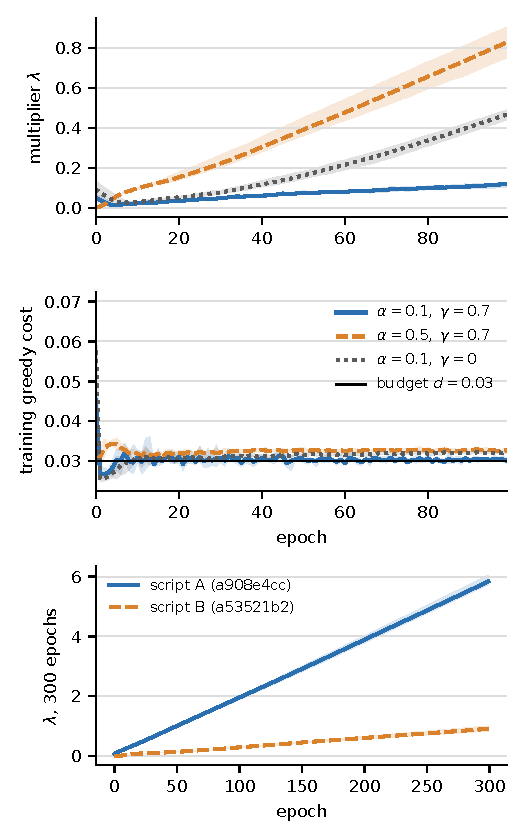
\includegraphics[width=\columnwidth]{figures/courbes_apprentissage.pdf}
\caption{Multiplier $\lambda$ (top) and greedy cost on the training windows (bottom) against the epoch for the three Safe-CQL configurations of the final evaluation: mean over five seeds and min--max band. Training data only, cost read in the training table. $\lambda$ does not converge by the criterion of the first diagnostic: none of the 15 runs satisfies it. The curves do not show a result on the test set.}% REG: E12P-c, E12P-e, CONV-a
\label{fig:curves}
\end{figure}

\subsection{Selection of the Conservatism Weight}
\label{sec:res_alpha}

No value of $\alpha$ is feasible under the frozen rule: in the direction from the second script to the first, the mean validation cost exceeds $d$ for every $\alpha$, from 0.0405 to 0.0504.% REG: E11-a
The two directions move in opposite ways with $\alpha$: from the first script to the second the cost decreases (0.0329 to 0.0227 at $\alpha=0.2$) and falls below $d$ from $\alpha=0.02$, whereas from the second to the first it increases (0.0405 to 0.0504); the validation reward decreases in both (9.12 to 7.86, and 10.06 to 7.90).% REG: E11-c
Averaging the two directions, as the fallback rule does, hides this opposition.% REG: E11-c
The fallback therefore keeps $\alpha=0.1$, with mean validation costs of 0.03470, 0.03440 and 0.03464 for $\alpha=0.05$, 0.1 and 0.2, a difference smaller than the spread between seeds of 0.0010 to 0.0021.% REG: E11-b
The choice of $\alpha=0.1$ is a consequence of the rule and not a finding that it is the best value.% REG: E11-b, NO-alpha
At $\alpha=0.1$ the validation reward of the $Q$-network is below that of the table-greedy built on the other script (8.056 against 10.352, and 8.321 against 11.370), and in the second direction its cost is higher as well (0.0454 against 0.0303).% REG: E11-e, NO-rl

\subsection{Transfer Between Scripts}
\label{sec:res_transfer}

The optimal policy built on the first script violates the budget when read in the tables of the second (a cost of 0.052 against 0.030), whereas the policy built on the second and read in the first has a cost of 0.0300 for the randomized solution and 0.0303 for the best deterministic one.% REG: TR-a
The failure is therefore verified in one direction only, and the other direction is within 1\% of $d$ and does not establish a violation.% REG: TR-b, TR-d
The interval of the transferred table-greedy cost is $[0.0147;0.0523]$ for the second-to-first direction (0.0303) and $[0.0146;0.0830]$ for the first-to-second (0.0520), and the shares of resamples at or below $d$ are 0.53 and 0.30.% REG: TR-e
With two scripts, a property of the pair cannot be separated from a general property.% REG: TR-c, TR-d

The direction of the transfer result is the same for every partition of the load tested, but its size depends on the partition.% REG: E13a2-b, E13a2-d
Over the partitions tested with integer edges, the transferred cost ranges from 0.0448 to 0.0520 in the first-to-second direction and from 0.0303 to 0.0357 in the other.% REG: E13a2-b
With quantile edges the first-to-second range is wider, from 0.0256 to 0.0520, because two partitions with two levels give 0.0256 (edge at 6.0) and 0.0463 (edge at 5.0); the result depends on where the edges are placed and not monotonically on the number of levels.% REG: E13a2-b, E13a2-d
The bootstrap intervals of the transferred cost contain $d$ in all the rows tested, 10 with quantile edges and 12 with integer edges, with widths of 0.034 to 0.068, so no difference between partitions is distinguishable from noise and none is ranked.% REG: E13a2-c
Between 52\% and 67\% of the cells (action by level) have an interval that contains $d$ with integer edges.% REG: E13a2-e
These analyses are on the training set, with two scripts, and do not choose a number of load levels: the main configuration keeps three levels and a window of 5\,s.% REG: E13a2-c, NO-bins, E13b-e

\subsection{Ablation $\gamma=0$}
\label{sec:res_gamma}

Setting $\gamma=0$ at $\alpha=0.1$ lowers the DM cost and the DM reward: on the whole test set the cost changes by $-0.0032$ and the reward by $-0.22$\,Mbps, and on the main script by $-0.0029$ and $-0.20$\,Mbps.% REG: E12-i
We read it as a trade-off, and not as an improvement.% REG: E12-i
The frozen criterion for a net improvement is a cost lower by more than twice the largest standard deviation across seeds.% REG: PREREG-a, E12-i
The margin is thin: the threshold is about 0.0032 on the main script for a difference of 0.0029, and about 0.0030 on the whole test set for a difference of 0.0032, so the criterion is not met on the main script and is met on the pooled set, which is 90\% that script.% REG: E12-i
The expectation of no net improvement therefore holds on the main script and does not hold on the pooled set, and we report it as it is.% REG: E12-i, E12-k
The difference is of the order of the variability across seeds (a standard deviation of the DM cost of 0.0016 and 0.0015 at $\gamma=0.7$, 0.0009 and 0.0008 at $\gamma=0$), and the criterion is arbitrary.% REG: E12-i
The ablation does not stop the drift of $\lambda$: the final $\lambda$ is 0.4398 to 0.4910, above the values at $\gamma=0.7$ and $\alpha=0.1$, and the diagnostic runs at $\alpha=0.5$ also show a larger $\lambda$ with $\gamma=0$.% REG: E12P-c, E2-c
We therefore do not conclude that $\gamma=0$ is the cause of the divergence of $\lambda$, nor that it is preferable.% REG: E2-c, E12-i

\subsection{What the Results Do Not Show}
\label{sec:claims_not}

\begin{itemize}
  \item \emph{No safety guarantee, and no lambda convergence.} No policy is demonstrated safe on the test script, no run satisfies the convergence criterion, and no value of $\alpha$ is feasible in validation.% REG: E12-e, E2-a, E12P-e, E11-a, NO-safe, NO-budget
  \item \emph{No superiority over a table.} A table built on the same cells has a higher DM reward and a lower DM cost than the learned agents on the main script, with the circularity of the DM estimate, and the $Q$-network is below a transferred table in validation.% REG: E12-f, E11-e, NO-rl
  \item \emph{No generalization.} The test is one script for 90\% of its reservations, the intervals are conditional on it, and the transfer was verified in one direction only.% REG: D6-b, BOOT-a, TR-d, NO-general
  \item \emph{No sequential control.} The data contain no action change, the agents are one-step selectors, and the estimators do not observe a change of action.% REG: D1-c, E12P-d, NO-seq
  \item \emph{No Near-RT validation.} The decision window is 5\,s, no window-sensitivity experiment was run, and the files do not allow the 10\,ms to 1\,s range.% REG: WIN-a, E13b-e, E13b-d, NO-nearrt
  \item \emph{No effect of the latency filter on the test.} The filter was measured on the training set only, and its effect on the test set is unknown.% REG: E13d-h, NO-filter
  \item \emph{No causal reading of the scheduler.} Always-PF has a higher cost than always-RR, but the scheduler cannot be separated from the execution block.% REG: E12-g, D7-b, NO-pfcause
\end{itemize}
